\documentclass[10.5pt,letterpaper]{article}
\usepackage[margin=0.75in]{geometry}
% \usepackage[T1]{fontenc}  % optional
\usepackage[utf8]{inputenc}
% \usepackage{lmodern}  % optional: uncomment if installed
% \usepackage{microtype} % optional
\usepackage{url}
\usepackage{graphicx}
\usepackage{booktabs}
\usepackage[hidelinks]{hyperref}
\usepackage{titlesec}
\usepackage{parskip}
\usepackage{enumitem}
\setlist{nosep,leftmargin=1.2em}

\titleformat{\section}{\large\bfseries}{}{0pt}{}
\titlespacing*{\section}{0pt}{0.9em}{0.2em}
\setlength{\parskip}{0.5em}
\urlstyle{same}

\begin{document}

\begin{center}
{\Large\bfseries CSC789 - AI Capstone Project Proposal}
\end{center}

\vspace{0.5em}
\noindent\textbf{Title:} Ontology-Based Scope Control for Conversational Agents: A Comparison with Prose and Blocklist Baselines

\noindent\textbf{Project track:} Track A: Research

\noindent\textbf{Student name:} Sravya Daggumalli (individual)

\section{Problem and Motivation}

Today it is common practice to tell LLM-based conversational agents what they may respond to through a free-text system prompt, and those instructions are usually a list of things the agent must not do. I ran into three problems with this while building agent guardrails on Azure AI Foundry for a personal project. There is no good way to check a prose prompt for contradictions or gaps except by trying questions one at a time. A blocklist can miss related cases its author did not anticipate prior. And permissions do not inherit: allowing a broad category does not reliably allow the narrower cases inside it unless each one is spelled out. Vendor guardrails cover fixed harm categories like hate or self-harm, not what a specific agent is supposed to be \emph{for}.

This project analyses whether a structured scope specification, an ontology where permissions are attached to concepts and a permission on a parent concept carries down to its children, makes better allow/refuse decisions than a prose prompt or a blocklist, and what it costs to build it.

\section{Related Work/Background}

There is a lot of recent work on runtime policy enforcement for LLM agents, including AgentSpec~\cite{agentspec}, FORGE~\cite{forge}, Agent Behavioral Contracts~\cite{abc}, and a recent paper on what runtime gates can enforce~\cite{ray2026}. Most of it focuses on which tools an agent may call rather than what it may talk about, and in the papers I reviewed none uses description logic or inheritance over a domain hierarchy. Ontology-based agent policy was tried in the 2000s (KAoS~\cite{kaos}, Rei~\cite{rei}) but has not been revisited for LLMs. NeMo Guardrails~\cite{nemo} comes closest with topical rails, but has no hierarchy. I did not find an empirical comparison of hierarchical scope specification against prose for conversational scope, which is the gap this project aims to fill.

\section{Research Questions}

\textbf{Q1.} Does an ontology with inherited permissions let fewer out-of-scope questions through than a prose prompt, a blocklist, or a flat topic list?

\textbf{Q2.} Does it do that without wrongly refusing more in-scope questions?

\textbf{Q3.} When it fails, is the failure in matching the question to a concept or in the policy itself?

\section{Project Challenges}

The hardest part is matching a user's question to the right concept in the ontology. If the match is wrong, the reasoning on top of it cannot help, so I will measure this by running the ontology once with automatic matching and once with the correct concept supplied from my labels. When nothing matches, the system refuses, which is right for out-of-scope questions but wrong for in-scope ones, and I will report how often that happens. The prose and blocklist baselines need to be strong for the comparison to mean anything, so I will tune them on a small held-out set before the test set is fixed. Finally, the Dallas export I have covers only one department, so I plan to pull the full request-type list through an aggregate query on the open data portal.

\section{Dataset}

I use the Dallas 311 Service Requests open data, October 2020 to present~\cite{dallas311}, in aggregate only: one grouped query returns department and request-type counts (435 rows, about 2.6 million requests). After stripping department codes from the type names, merging duplicate department labels, and dropping test records, 270 services remain across 23 departments, 201 with at least 50 requests (Fig.~\ref{fig:taxonomy}). No individual records or locations are used.

\begin{figure}[t]
\centering
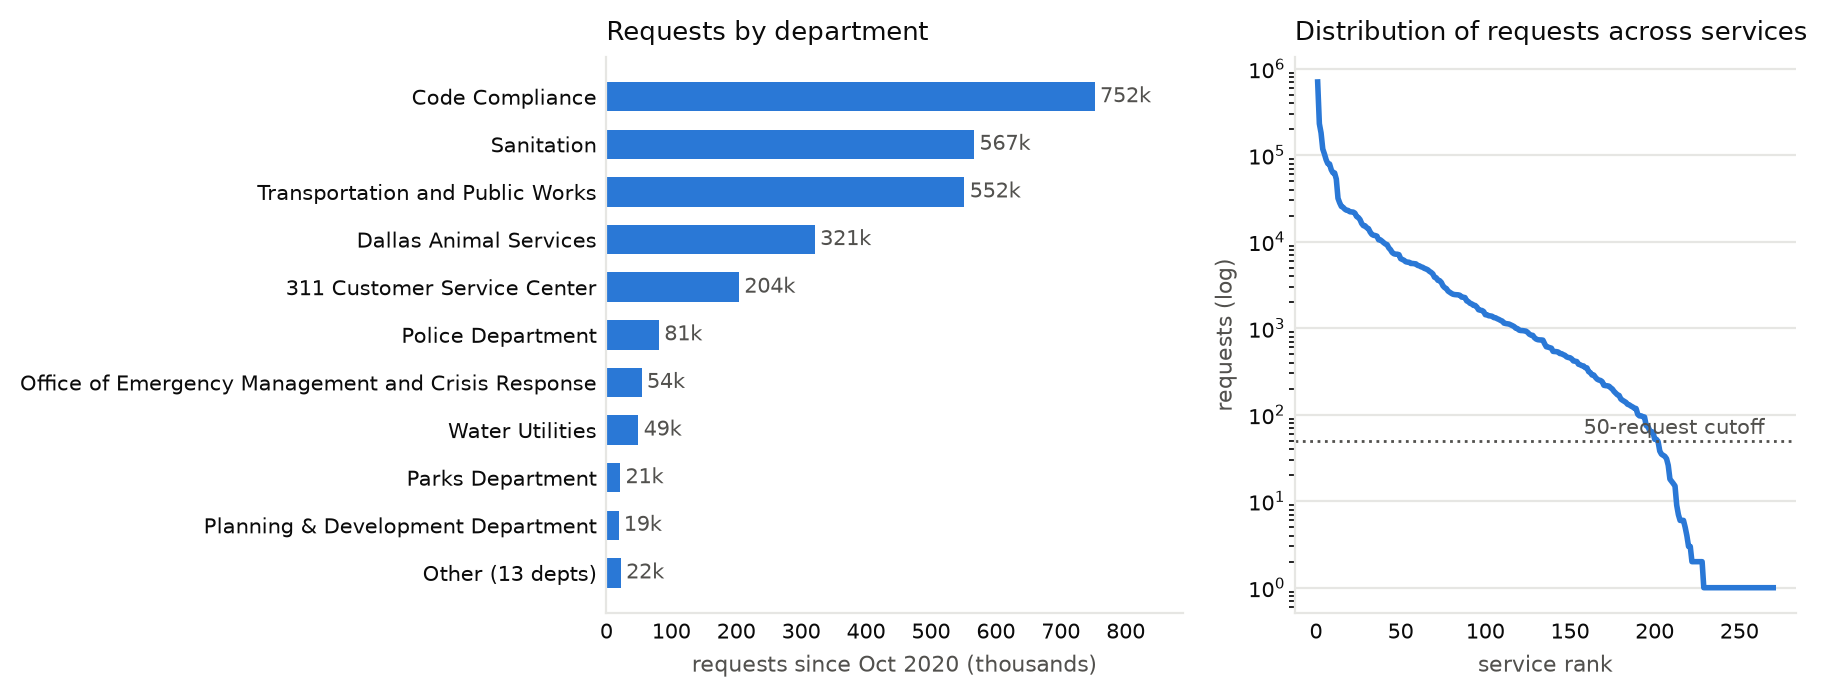
\includegraphics[width=\columnwidth]{figures/taxonomy_overview.png}
\caption{Dallas 311 requests by department (left) and across all services sorted by volume, log scale (right).}
\label{fig:taxonomy}
\end{figure}

The pilot evaluation set has 42 hand-written questions in four groups: direct (11), inheritance-dependent (10), paraphrase (10), and out-of-scope (11), each labeled allow or refuse with its concept. The out-of-scope group is built from near misses that reuse 311 vocabulary. The full 160-question set with a second labeler is scheduled for Week 6.

\section{Proposed AI Approach}

Each apporach takes a question and returns \textbf{allow} or \textbf{refuse} with a short reason. No chat interface or answer text is built and the decision is used as a measure.

\begin{itemize}\setlength{\itemsep}{1pt}
  \item \textbf{(A) Prose prompt.} A system prompt describing what the assistant covers, run through a small hosted LLM.
  \item \textbf{(B) Prose + blocklist.} Same prompt plus an explicit list of forbidden topics.
  \item \textbf{(R) Flat list.} The same concepts as the ontology, no hierarchy, matched by embedding similarity. No LLM.
  \item \textbf{(C) Ontology (proposed).} 60--100 concepts, three levels deep, built in Prot\'eg\'e from the Dallas request types, each marked permitted or denied.
  \begin{itemize}\setlength{\itemsep}{0pt}
    \item Match the question to the closest concept with a small sentence-embedding model (e.g.\ \texttt{bge-small-en-v1.5}); no match above threshold means refuse.
    \item Walk the concept's ancestors in Python with a most-specific-wins rule, so a parent's permission covers its children unless a child overrides it.
    \item An OWL reasoner via \texttt{owlready2}~\cite{owlready} keeps the hierarchy consistent and flags any concept marked both permitted and denied.
  \end{itemize}
  \item \textbf{(D) Ontology with gold concept.} Same as C but the correct concept comes from my labels, skipping matching. A diagnostic upper bound, not a usable system.
\end{itemize}

\subsection{Baselines and pilot result}

The primary baseline is the prose system prompt, which is what AgentSpec~\cite{agentspec}, FORGE~\cite{forge}, and NeMo Guardrails~\cite{nemo} all compare against and what practitioners deploy. The second baseline is a flat list of concepts matched by embedding similarity, the same approach NeMo's topical rails use. It is built from same concepts, embedding model, and threshold as the ontology arm, so the only difference between the flat list and the ontology arm is the heirarchy. Table~\ref{tab:baseline} shows both on the pilot set. The prompt model (gpt-6-luna) does not accept a temperature setting, so the final experiment will use three runs with majority voting.

\begin{table}[h]
\centering
\caption{Baseline results on the 42-question pilot set (31 in-scope, 11 out-of-scope).}
\label{tab:baseline}
\begin{tabular}{lcc}
\toprule
Baseline & Out-of-scope allowed & In-scope refused \\
\midrule
Flat list (R) & 5/11 & 0/31 \\
Prompt (A)    & 1/11 & 5/31 \\
\bottomrule
\end{tabular}
\end{table}

The two fail in opposite directions. The flat matcher refused no in-scope questions but allowed 5 of 11 near misses. The prompt allowed only one, but refused 5 in-scope questions, each time because it classified a hazardous but routine report (bent guardrail, low limb, chained dog) as an emergency. This suggests the ontology will need hazardous-but-routine concepts under permitted parents, separate from a denied Emergency concept.


\section{Evaluation Plan}

\begin{itemize}\setlength{\itemsep}{1pt}
  \item \textbf{Metrics}, per approach and per question group on the 120 test questions: out-of-scope questions allowed; in-scope questions refused; for the ontology, how often a question matched any concept and how often an acceptable one.
  \item \textbf{Comparison:} McNemar's test between approaches (all see the same questions), plus a table of which questions each approach got wrong.
  \item \textbf{Qualitative:} the inheritance path used for questions that depend on it; the reasoner catching a concept marked both permitted and denied before any question is run.
  \item \textbf{Expected result:} the ontology does best on inheritance-dependent questions, loses some on reworded questions to matching errors, and differs little on questions that name a service directly.
  \item \textbf{Schedule:} taxonomy, questions, and ontology by Week 6; runs and analysis Weeks 7-9; and a report after that. API should cost under \$30; everything else runs on my computer.
\end{itemize}

\section{Expected Contribution / Value}

A small, reproducible comparison of prose, blocklist, flat-list, and hierarchical scope policies on a constructed 311 benchmark, produced with the question set and ontology. It will show whether inheritance helps, how much is lost to automatic matching, and that a structured policy can be checked for conflicts before use. If a well-tuned prompt matches the ontology at this scale, that is still a useful result about when a formal specification is worth the effort.

\begin{thebibliography}{10}
\setlength{\itemsep}{0pt}
\scriptsize

\bibitem{agentspec} H.~Wang, C.~M. Poskitt, and J.~Sun. AgentSpec: Customizable Runtime Enforcement for Safe and Reliable LLM Agents. \emph{Proc.\ ICSE 2026}. arXiv:2503.18666.

\bibitem{forge} N.~Palumbo, S.~Choudhary, J.~Choi, G.~Amir, P.~Chalasani, and S.~Jha. Formal Policy Enforcement for Real-World Agentic Systems. arXiv:2602.16708, 2026.

\bibitem{abc} V.~P. Bhardwaj. Agent Behavioral Contracts: Formal Specification and Runtime Enforcement for Reliable Autonomous AI Agents. arXiv:2602.22302, 2026.

\bibitem{ray2026} S.~Ray. What Can Be Enforced? A Theory of Certified Runtime Safety for Tool-Using Agents. arXiv:2607.22868, 2026.

\bibitem{kaos} A.~Uszok, J.~M. Bradshaw, et al. KAoS Policy and Domain Services: Toward a Description-Logic Approach to Policy Representation, Deconfliction, and Enforcement. \emph{IEEE POLICY 2003}.

\bibitem{rei} L.~Kagal, T.~Finin, and A.~Joshi. A Policy Language for a Pervasive Computing Environment. \emph{IEEE POLICY 2003}.

\bibitem{nemo} T.~Rebedea et al. NeMo Guardrails: A Toolkit for Controllable and Safe LLM Applications with Programmable Rails. \emph{EMNLP 2023 System Demonstrations}.

\bibitem{owlready} J.-B. Lamy. Owlready: Ontology-Oriented Programming in Python with Automatic Classification and High Level Constructs for Biomedical Ontologies. \emph{Artificial Intelligence in Medicine} 80:11--28, 2017.

\bibitem{dallas311} City of Dallas. 311 Service Requests October 1, 2020 to Present [dataset]. Dallas OpenData, id d7e7-envw. Accessed Sep. 2026. \url{https://www.dallasopendata.com/Services/311-Service-Requests/d7e7-envw}


\end{thebibliography}

\vspace{0.3em}

\end{document}
